% File: result.tex
% Date: Wed Jun 17 21:33:03 2015 +0800
% Author: Yuxin Wu <ppwwyyxxc@gmail.com>

\section{More Results}
\begin{figure}[H]
  \centering
  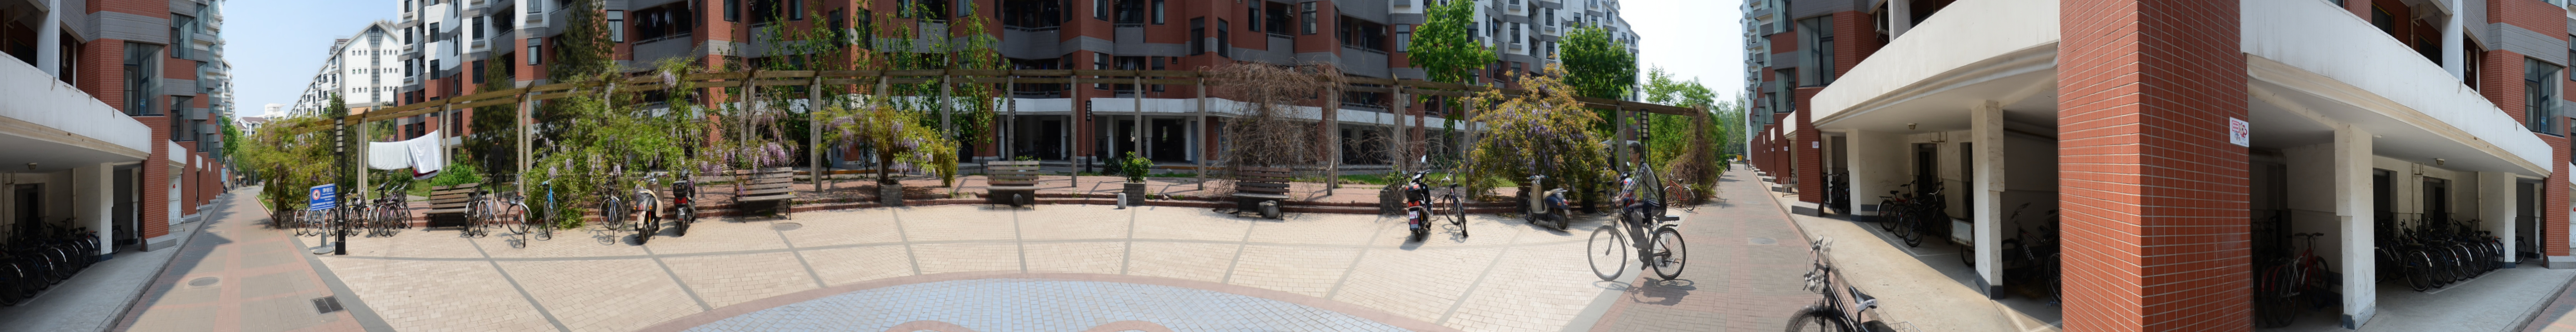
\includegraphics[width=\textwidth]{res/results/apartment.jpg}
  \caption{Zijing Apartment in Tsinghua University}
\end{figure}

\begin{figure}[H]
  \centering
  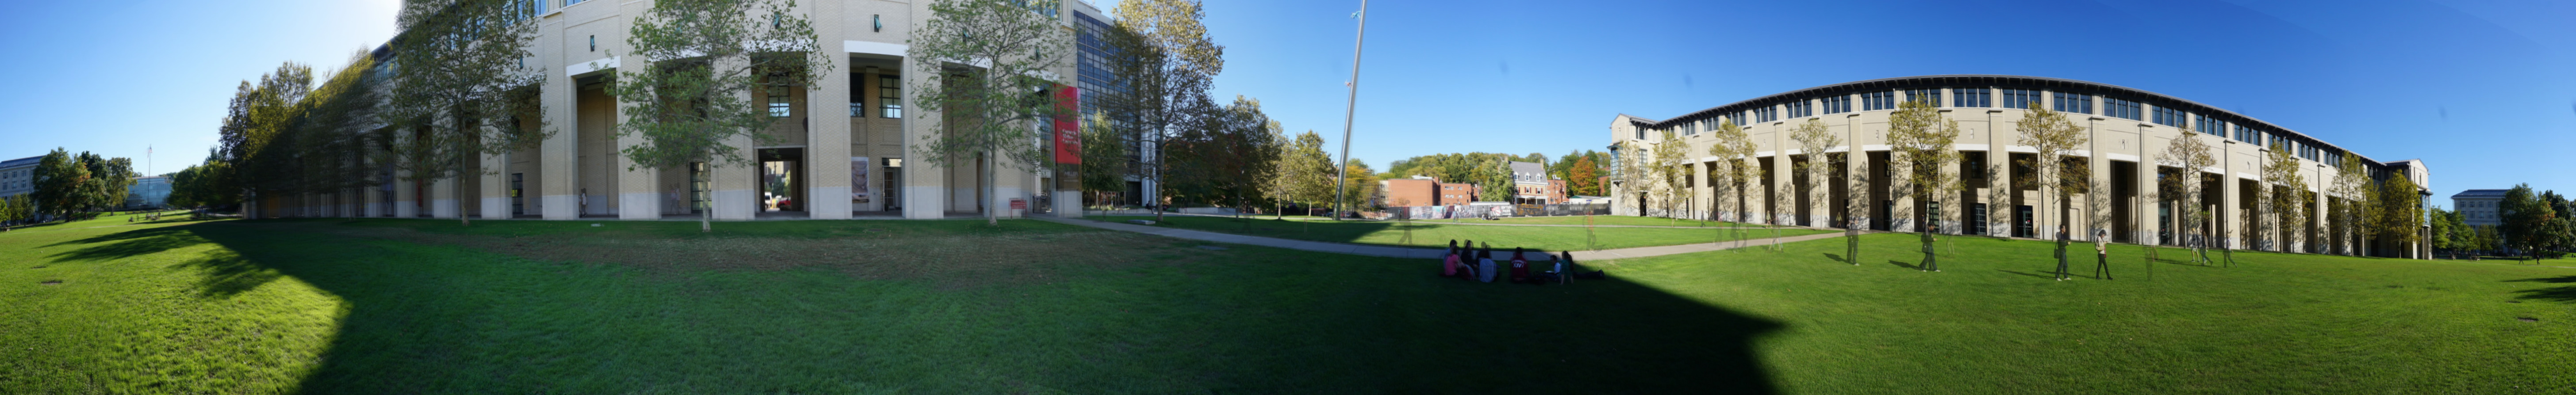
\includegraphics[width=\textwidth]{res/results/CMU0-cyl.jpg}
  \caption{Carnegie Mellon University}
\end{figure}

\begin{figure}[H]
  \centering
  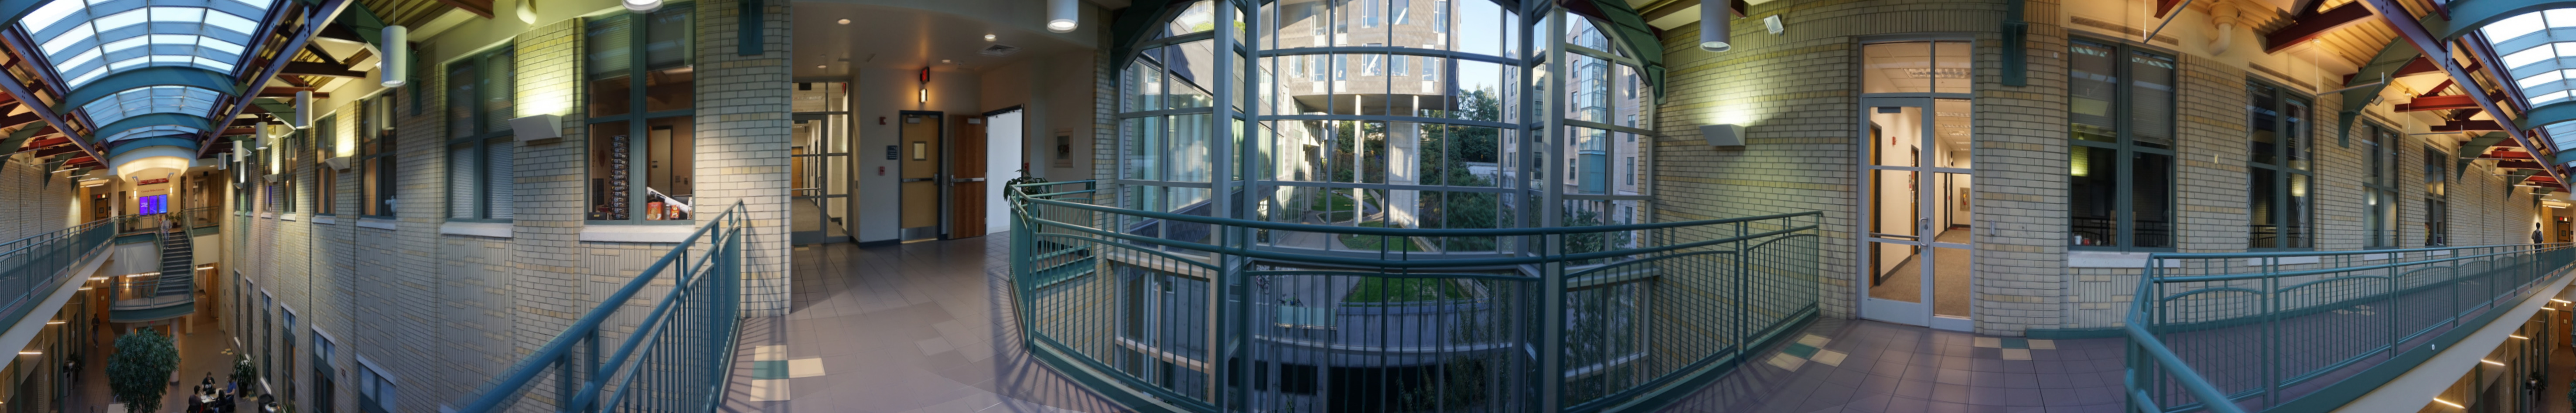
\includegraphics[width=\textwidth]{res/results/NSH-cyl.jpg}
  \caption{Newell Simon Hall at CMU (this is hard since objects are close to camera)}
\end{figure}
\begin{figure}[H]
  \centering
  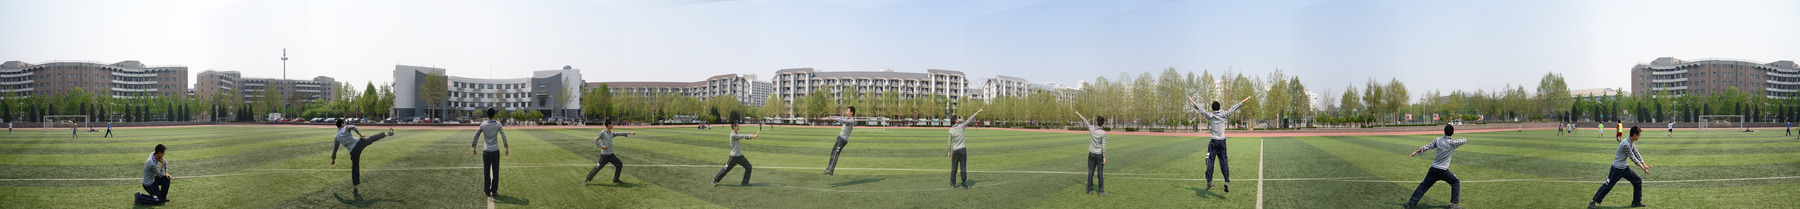
\includegraphics[width=\textwidth]{res/results/myself.jpg}
  \caption{me being silly}
\end{figure}

In camera estimation mode, no translation is the only requirement on camera.
So we can even build wider-angle panorama:
\begin{figure}[H]
  \centering
  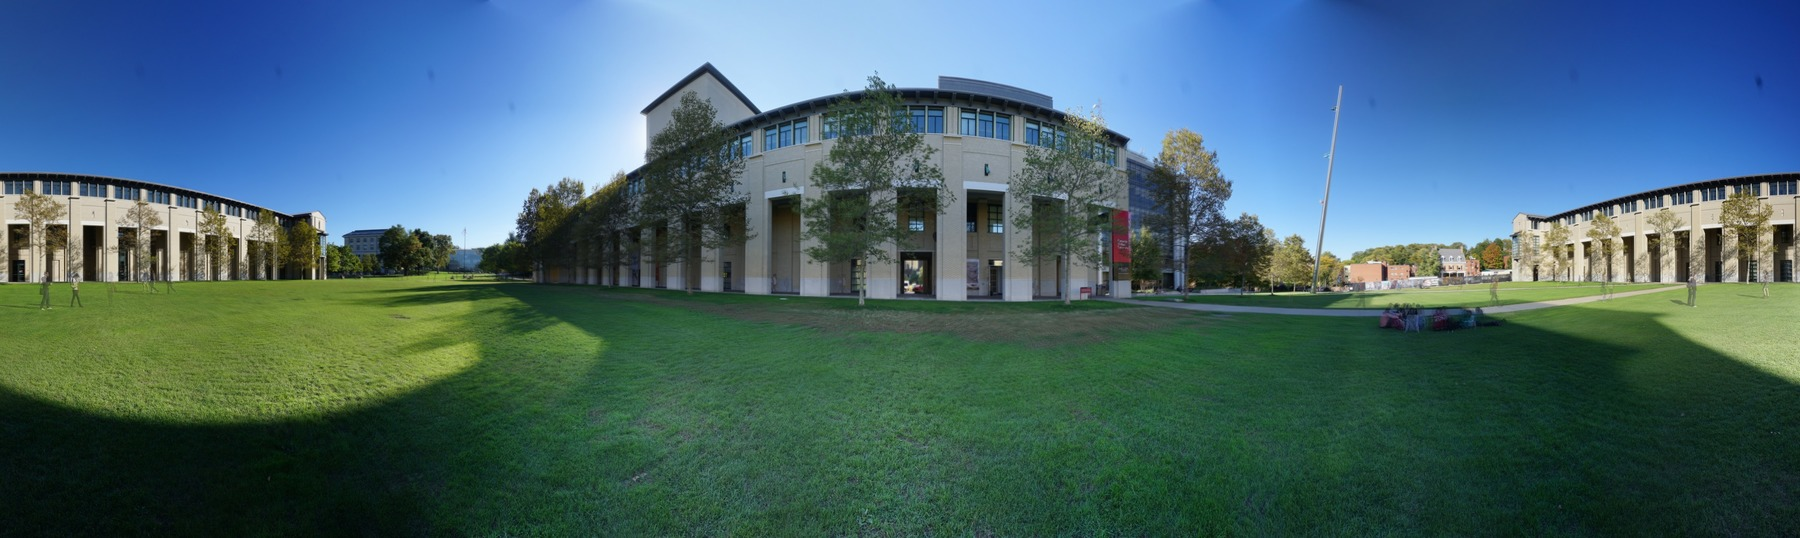
\includegraphics[width=\textwidth]{res/results/CMU0-all.jpg}
  \caption{CMU stitched with 38 images.}
\end{figure}


\newpage
By adding a polar transformation on the above result, we can simply turn it into this:

%\begin{figure}[H]
  %\centering
  %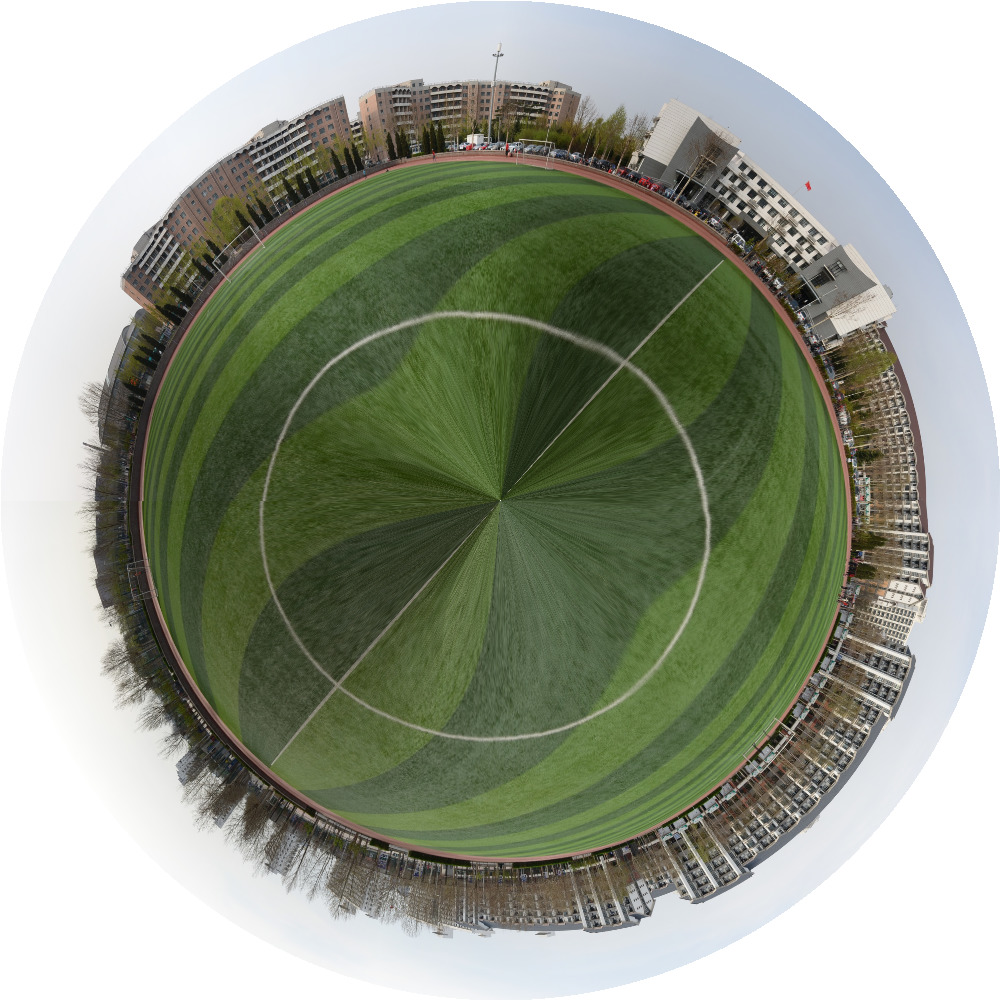
\includegraphics[width=\textwidth]{res/results/planet.jpg}
  %\caption{Soccer Field}
%\end{figure}

\begin{figure}[H]
  \centering
  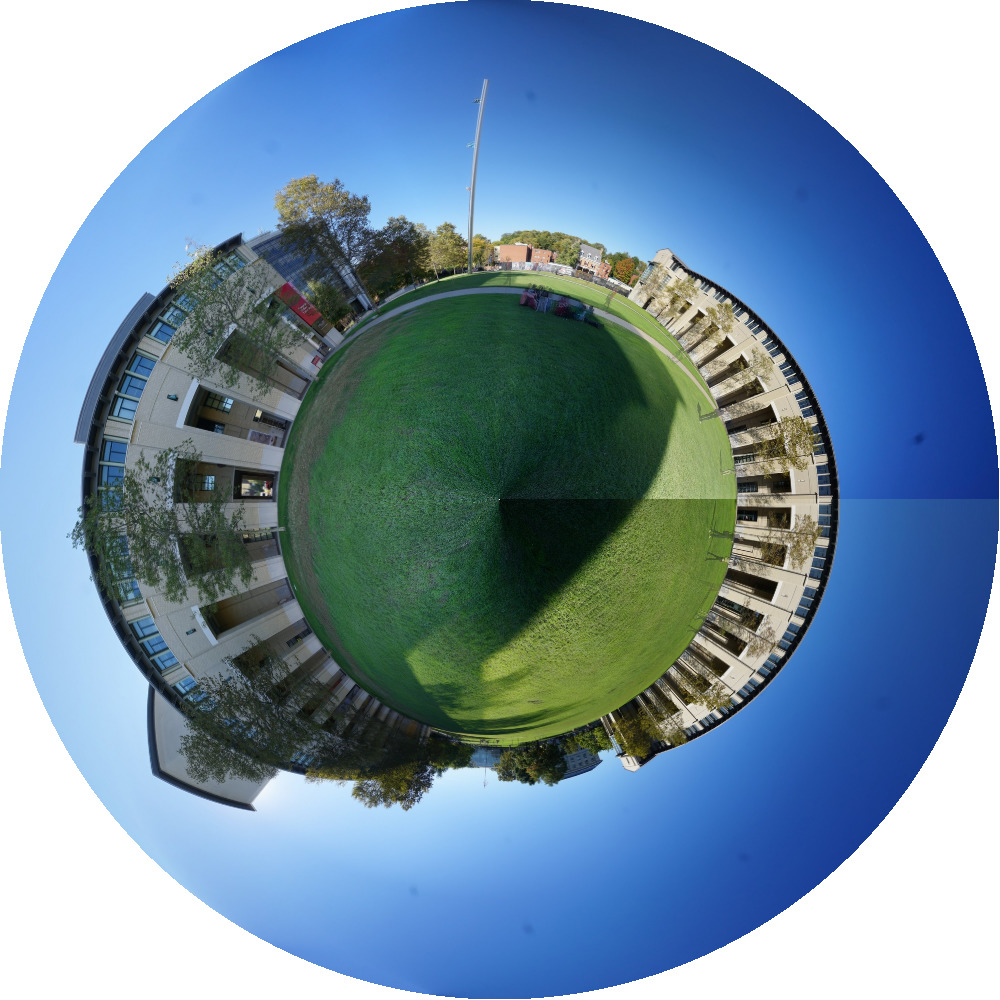
\includegraphics[width=\textwidth]{res/results/apple.jpg}
\end{figure}
